\documentclass[letter,10pt,twoside]{article}

\usepackage[spanish,es-nodecimaldot]{babel}
\usepackage[utf8]{inputenc}

\renewcommand{\familydefault}{\sfdefault}
\usepackage[T1]{fontenc}
\usepackage{textcomp}

\usepackage{framed}
\usepackage[svgnames]{xcolor}
\colorlet{shadecolor}{Gainsboro!50}

\usepackage{enumitem}
\usepackage{graphicx}
\usepackage{pstricks}

\usepackage{anysize}
\marginsize{3cm}{2cm}{2cm}{3cm}

\usepackage{float}
\usepackage{siunitx}
\usepackage{amsmath}
\usepackage{array}

\usepackage{multicol}
\usepackage{pifont}

\usepackage{fancyhdr}
\usepackage{lastpage}
\pagestyle{fancy}
\fancyhf{}
\fancyhead[LE,RO]{Resistencia de los Materiales}
\fancyfoot[CO,CE]{\thepage\ de \pageref{LastPage}}

\special{papersize=215.9mm,279.4mm}

\usepackage[
    pdfauthor={Carlos Eduardo Caballero Burgoa},%
    pdftitle={Resistencia de los Materiales},%
    pdfsubject={Practica 03},%
    colorlinks,%
    citecolor=black,%
    filecolor=black,%
    linkcolor=black,%
    urlcolor=black,
    breaklinks]{hyperref}
\usepackage{breakurl}

\newcommand{\blankpage}{
\newpage
\thispagestyle{empty}
\mbox{}
\newpage
}

\renewcommand{\arraystretch}{1.2}

\begin{document}

\begin{titlepage}
\begin{center}
{\Large UNIVERSIDAD MAYOR DE SAN SIMÓN}\\
\vspace*{0.15cm}
{\large FACULTAD DE CIENCIAS Y TECNOLOGÍA}\\
\vspace*{9.0cm}
{\Large \textbf{PRACTICA No. 3}}\\
\end{center}

\vspace*{7.4cm}
\leftskip=7.95cm
\noindent
\textbf{Estudiante:}\\
Caballero Burgoa, Carlos Eduardo.\\
\textbf{Carrera:}\\
Ingeniería Electromecánica.\\
\newline
\textbf{Docente:}\\
Ing. Guido Gómez Ugarte.\\
\newline
\textbf{Fecha de entrega:} 11 de Octubre del 2022.\\

\end{titlepage}

\blankpage

\colorbox{blue!25}{\textbf{PROBLEMA 1:}}

\begin{enumerate}[label=\alph*)]
    \item Trazar el circulo de \emph{Mohr}.
    \item Hallar: $\sigma_{\text{max}}$, $\sigma_{\text{min}}$, $\alpha$ y
        $\beta$.
    \item Las secciones principales.
\end{enumerate}

\begin{figure}[H]
\centering
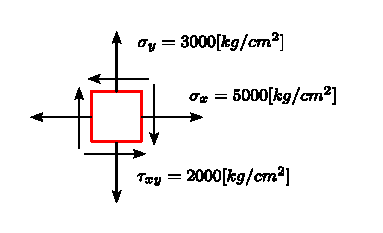
\includegraphics[scale=1.2]{resources/f10.eps}
\end{figure}

\textbf{\underline{Solución}:} \\

a) Circulo de \emph{Mohr}:

\begin{equation*}
    \sigma_x = 5000[\text{kg}/\text{cm}^2]
\end{equation*}
\begin{equation*}
    \sigma_y = 3000[\text{kg}/\text{cm}^2]
\end{equation*}
\begin{equation*}
    \tau_{xy} = 2000[\text{kg}/\text{cm}^2]
\end{equation*}

\begin{figure}[H]
\centering
\includegraphics[scale=1.2]{resources/f11.eps}
\end{figure}

b) $\sigma_{\text{max}}$, $\sigma_{\text{min}}$, $\alpha$ y $\beta$.

\begin{equation*}
    \sigma_0 = \frac{\sigma_x + \sigma_y}{2}
             = \frac{8000}{2}
             = 4000[\text{kg}/\text{cm}^2]
\end{equation*}
\begin{equation*}
    a = \frac{\sigma_x - \sigma_y}{2}
      = \frac{2000}{2}
      = 1000[\text{kg}/\text{cm}^2]
\end{equation*}
\begin{equation*}
    b = \tau_{xy}
      = 2000[\text{kg}/\text{cm}^2]
\end{equation*}
\begin{equation*}
    R = \sqrt{a^2 + b^2}
      = \sqrt{1000^2 + 2000^2}
      = 2236.07
\end{equation*}
\begin{equation*}
    \sigma_{\text{max}} = \sigma_0 + R
                        = 6236.08[\text{kg}/\text{cm}^2]
\end{equation*}
\begin{equation*}
    \sigma_{\text{min}} = \sigma_0 - R
                        = 1763.93[\text{kg}/\text{cm}^2]
\end{equation*}
\begin{equation*}
    \tau_{\text{max}} = R
                      = 2236.07[\text{kg}/\text{cm}^2]
\end{equation*}
\begin{equation*}
    \text{tan}\,2\alpha = \frac{b}{a}
                        = \frac{2000}{1000}
                        = 1000
\end{equation*}
\begin{equation*}
    \alpha = \frac{\text{tan}^{-1}(1000)}{2}
           = 31.72^\circ
\end{equation*}
\begin{equation*}
    2\alpha + 2\beta = 90^\circ
\end{equation*}
\begin{equation*}
    \beta = \frac{90 - 2\alpha}{2}
          = 13.28^\circ
\end{equation*}

\begin{equation*}
\boxed{
    \begin{array}{l}
        \sigma_{\text{max}} = 6236.08[\text{kg}/\text{cm}^2] \\
        \sigma_{\text{min}} = 1763.93[\text{kg}/\text{cm}^2] \\
        \alpha = 31.72^\circ \\
        \beta = 13.28^\circ
    \end{array}
}
\end{equation*}

c) 

\begin{figure}[H]
\centering
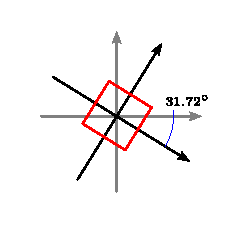
\includegraphics[scale=1.6]{resources/f12.eps}
\end{figure}

\begin{figure}[H]
\centering
\includegraphics[scale=1.6]{resources/f13.eps}
\end{figure}

\newpage

\colorbox{blue!25}{\textbf{PROBLEMA 2:}}

\begin{enumerate}[label=\alph*)]
    \item Trazar el circulo de \emph{Mohr}.
    \item Hallar: $\sigma_{\text{max}}$, $\sigma_{\text{min}}$, $\alpha$ y
        $\beta$.
    \item Las secciones principales.
\end{enumerate}

\begin{figure}[H]
\centering
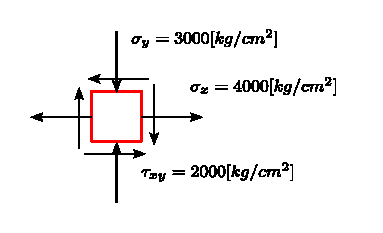
\includegraphics[scale=1.2]{resources/f20.eps}
\end{figure}

\textbf{\underline{Solución}:} \\

a) Circulo de \emph{Mohr}:

\begin{equation*}
    \sigma_x = 4000[\text{kg}/\text{cm}^2]
\end{equation*}
\begin{equation*}
    \sigma_y = -3000[\text{kg}/\text{cm}^2]
\end{equation*}
\begin{equation*}
    \tau_{xy} = 2000[\text{kg}/\text{cm}^2]
\end{equation*}

\begin{figure}[H]
\centering
\includegraphics[scale=1.2]{resources/f21.eps}
\end{figure}

b) $\sigma_{\text{max}}$, $\sigma_{\text{min}}$, $\alpha$ y $\beta$.

\begin{equation*}
    \sigma_0 = \frac{\sigma_x + \sigma_y}{2}
             = \frac{4000 - 3000}{2}
             = 500[\text{kg}/\text{cm}^2]
\end{equation*}
\begin{equation*}
    a = \frac{\sigma_x - \sigma_y}{2}
      = \frac{4000 - (-3000)}{2}
      = 3500[\text{kg}/\text{cm}^2]
\end{equation*}
\begin{equation*}
    b = \tau_{xy}
      = 2000[\text{kg}/\text{cm}^2]
\end{equation*}
\begin{equation*}
    R = \sqrt{a^2 + b^2}
      = \sqrt{3500^2 + 2000^2}
      = 4031.13
\end{equation*}
\begin{equation*}
    \sigma_{\text{max}} = \sigma_0 + R
                        = 4531.13[\text{kg}/\text{cm}^2]
\end{equation*}
\begin{equation*}
    \sigma_{\text{min}} = \sigma_0 - R
                        = -3531.13[\text{kg}/\text{cm}^2]
\end{equation*}
\begin{equation*}
    \tau_{\text{max}} = R
                      = 4031.13[\text{kg}/\text{cm}^2]
\end{equation*}
\begin{equation*}
    \text{tan}\,2\alpha = \frac{b}{a}
                        = \frac{2000}{3500}
                        = \frac{4}{7}
\end{equation*}
\begin{equation*}
    \alpha = \frac{\text{tan}^{-1}(0.5714)}{2}
           = 14.87^\circ
\end{equation*}
\begin{equation*}
    2\alpha + 2\beta = 90^\circ
\end{equation*}
\begin{equation*}
    \beta = \frac{90 - 2\alpha}{2}
          = 30.13^\circ
\end{equation*}

\begin{equation*}
\boxed{
    \begin{array}{l}
        \sigma_{\text{max}} = 4531.13[\text{kg}/\text{cm}^2] \\
        \sigma_{\text{min}} = -3531.13[\text{kg}/\text{cm}^2] \\
        \alpha = 14.87^\circ \\
        \beta = 30.13^\circ
    \end{array}
}
\end{equation*}

c) 

\begin{figure}[H]
\centering
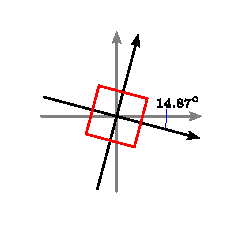
\includegraphics[scale=1.6]{resources/f22.eps}
\end{figure}

\begin{figure}[H]
\centering
\includegraphics[scale=1.6]{resources/f23.eps}
\end{figure}

\newpage

\colorbox{blue!25}{\textbf{PROBLEMA 3:}}

\begin{enumerate}[label=\alph*)]
    \item Trazar el circulo de \emph{Mohr}.
    \item Hallar: $\sigma_{\text{max}}$, $\sigma_{\text{min}}$, $\alpha$ y
        $\beta$.
    \item Las secciones principales.
\end{enumerate}

\begin{figure}[H]
\centering
\includegraphics[scale=1.2]{resources/f30.eps}
\end{figure}

\textbf{\underline{Solución}:} \\

a) Circulo de \emph{Mohr}:

\begin{equation*}
    \sigma_x = -3000[\text{kg}/\text{cm}^2]
\end{equation*}
\begin{equation*}
    \sigma_y = -5000[\text{kg}/\text{cm}^2]
\end{equation*}
\begin{equation*}
    \tau_{xy} = 2000[\text{kg}/\text{cm}^2]
\end{equation*}

\begin{figure}[H]
\centering
\includegraphics[scale=1.2]{resources/f31.eps}
\end{figure}

b) $\sigma_{\text{max}}$, $\sigma_{\text{min}}$, $\alpha$ y $\beta$.

\begin{equation*}
    \sigma_0 = \frac{\sigma_x + \sigma_y}{2}
             = \frac{-3000 - 5000}{2}
             = -4000[\text{kg}/\text{cm}^2]
\end{equation*}
\begin{equation*}
    a = \frac{\sigma_x - \sigma_y}{2}
      = \frac{-3000 - (-5000)}{2}
      = 1000[\text{kg}/\text{cm}^2]
\end{equation*}
\begin{equation*}
    b = \tau_{xy}
      = 2000[\text{kg}/\text{cm}^2]
\end{equation*}
\begin{equation*}
    R = \sqrt{a^2 + b^2}
      = \sqrt{1000^2 + 2000^2}
      = 2236.07
\end{equation*}
\begin{equation*}
    \sigma_{\text{max}} = \sigma_0 + R
                        = -1763.93[\text{kg}/\text{cm}^2]
\end{equation*}
\begin{equation*}
    \sigma_{\text{min}} = \sigma_0 - R
                        = -6236.07[\text{kg}/\text{cm}^2]
\end{equation*}
\begin{equation*}
    \tau_{\text{max}} = R
                      = 2236.07[\text{kg}/\text{cm}^2]
\end{equation*}
\begin{equation*}
    \text{tan}\,2\alpha = \frac{b}{a}
                        = \frac{2000}{1000}
                        = 2
\end{equation*}
\begin{equation*}
    \alpha = \frac{\text{tan}^{-1}(2)}{2}
           = 31.72^\circ
\end{equation*}
\begin{equation*}
    2\alpha + 2\beta = 90^\circ
\end{equation*}
\begin{equation*}
    \beta = \frac{90 - 2\alpha}{2}
          = 13.28^\circ
\end{equation*}

\begin{equation*}
\boxed{
    \begin{array}{l}
        \sigma_{\text{max}} = -1763.93[\text{kg}/\text{cm}^2] \\
        \sigma_{\text{min}} = -6236.07[\text{kg}/\text{cm}^2] \\
        \alpha = 31.72^\circ \\
        \beta = 13.28^\circ
    \end{array}
}
\end{equation*}

c) 

\begin{figure}[H]
\centering
\includegraphics[scale=1.6]{resources/f32.eps}
\end{figure}

\begin{figure}[H]
\centering
\includegraphics[scale=1.6]{resources/f33.eps}
\end{figure}

\newpage

\colorbox{blue!25}{\textbf{PROBLEMA 4:}}

\begin{enumerate}[label=\alph*)]
    \item Trazar el circulo de \emph{Mohr}.
    \item Hallar: $\sigma_{\text{max}}$, $\sigma_{\text{min}}$, $\alpha$ y
        $\beta$.
    \item Las secciones principales.
\end{enumerate}

\begin{figure}[H]
\centering
\includegraphics[scale=1.2]{resources/f40.eps}
\end{figure}

\textbf{\underline{Solución}:} \\

a) Circulo de \emph{Mohr}:

\begin{equation*}
    \sigma_x = 5000[\text{kg}/\text{cm}^2]
\end{equation*}
\begin{equation*}
    \sigma_y = 3000[\text{kg}/\text{cm}^2]
\end{equation*}
\begin{equation*}
    \tau_{xy} = 0[\text{kg}/\text{cm}^2]
\end{equation*}

\begin{figure}[H]
\centering
\includegraphics[scale=1.2]{resources/f41.eps}
\end{figure}

b) $\sigma_{\text{max}}$, $\sigma_{\text{min}}$, $\alpha$ y $\beta$.

\begin{equation*}
    \sigma_0 = \frac{\sigma_x + \sigma_y}{2}
             = \frac{5000 + 3000}{2}
             = 4000[\text{kg}/\text{cm}^2]
\end{equation*}
\begin{equation*}
    a = \frac{\sigma_x - \sigma_y}{2}
      = \frac{5000 - 3000}{2}
      = 1000[\text{kg}/\text{cm}^2]
\end{equation*}
\begin{equation*}
    b = \tau_{xy}
      = 0[\text{kg}/\text{cm}^2]
\end{equation*}
\begin{equation*}
    R = \sqrt{a^2 + b^2}
      = \sqrt{1000^2 + 0^2}
      = 1000
\end{equation*}
\begin{equation*}
    \sigma_{\text{max}} = \sigma_0 + R
                        = 5000[\text{kg}/\text{cm}^2]
\end{equation*}
\begin{equation*}
    \sigma_{\text{min}} = \sigma_0 - R
                        = 3000[\text{kg}/\text{cm}^2]
\end{equation*}
\begin{equation*}
    \tau_{\text{max}} = R
                      = 1000[\text{kg}/\text{cm}^2]
\end{equation*}
\begin{equation*}
    \text{tan}\,2\alpha = \frac{b}{a}
                        = \frac{0}{1000}
                        = 0
\end{equation*}
\begin{equation*}
    \alpha = \frac{\text{tan}^{-1}(0)}{2}
           = 0^\circ
\end{equation*}
\begin{equation*}
    2\alpha + 2\beta = 90^\circ
\end{equation*}
\begin{equation*}
    \beta = \frac{90 - 2\alpha}{2}
          = 45^\circ
\end{equation*}

\begin{equation*}
\boxed{
    \begin{array}{l}
        \sigma_{\text{max}} = 5000[\text{kg}/\text{cm}^2] \\
        \sigma_{\text{min}} = 3000[\text{kg}/\text{cm}^2] \\
        \alpha = 0^\circ \\
        \beta = 45^\circ
    \end{array}
}
\end{equation*}

c) 

\begin{figure}[H]
\centering
\includegraphics[scale=1.6]{resources/f42.eps}
\end{figure}

\begin{figure}[H]
\centering
\includegraphics[scale=1.6]{resources/f43.eps}
\end{figure}

\newpage

\colorbox{blue!25}{\textbf{PROBLEMA 5:}}

\begin{enumerate}[label=\alph*)]
    \item Trazar el circulo de \emph{Mohr}.
    \item Hallar: $\sigma_{\text{max}}$, $\sigma_{\text{min}}$, $\alpha$ y
        $\beta$.
    \item Las secciones principales.
\end{enumerate}

\begin{figure}[H]
\centering
\includegraphics[scale=1.2]{resources/f50.eps}
\end{figure}

\textbf{\underline{Solución}:} \\

a) Circulo de \emph{Mohr}:

\begin{equation*}
    \sigma_x = 3000[\text{kg}/\text{cm}^2]
\end{equation*}
\begin{equation*}
    \sigma_y = 3000[\text{kg}/\text{cm}^2]
\end{equation*}

\begin{figure}[H]
\centering
\includegraphics[scale=1.2]{resources/f51.eps}
\end{figure}

b) $\sigma_{\text{max}}$, $\sigma_{\text{min}}$, $\alpha$ y $\beta$.

\begin{equation*}
    \sigma_0 = \frac{\sigma_x + \sigma_y}{2}
             = \frac{3000 + 3000}{2}
             = 3000[\text{kg}/\text{cm}^2]
\end{equation*}
\begin{equation*}
    a = \frac{\sigma_x - \sigma_y}{2}
      = \frac{3000 - 3000}{2}
      = 0[\text{kg}/\text{cm}^2]
\end{equation*}
\begin{equation*}
    b = \tau_{xy}
      = 0[\text{kg}/\text{cm}^2]
\end{equation*}
\begin{equation*}
    R = \sqrt{a^2 + b^2}
      = \sqrt{0^2 + 0^2}
      = 0
\end{equation*}
\begin{equation*}
    \sigma_{\text{max}} = \sigma_0 + R
                        = 3000[\text{kg}/\text{cm}^2]
\end{equation*}
\begin{equation*}
    \sigma_{\text{min}} = \sigma_0 - R
                        = 3000[\text{kg}/\text{cm}^2]
\end{equation*}
\begin{equation*}
    \tau_{\text{max}} = R
                      = 0[\text{kg}/\text{cm}^2]
\end{equation*}
\begin{equation*}
    \alpha = \text{indeterminado}
\end{equation*}
\begin{equation*}
    \beta = \text{indeterminado}
\end{equation*}

\begin{equation*}
\boxed{
    \begin{array}{l}
        \sigma_{\text{max}} = 3000[\text{kg}/\text{cm}^2] \\
        \sigma_{\text{min}} = 3000[\text{kg}/\text{cm}^2] \\
        \alpha = \text{indeterminado} \\
        \beta = \text{indeterminado}
    \end{array}
}
\end{equation*}

\newpage

\colorbox{blue!25}{\textbf{PROBLEMA 6:}}

\begin{enumerate}[label=\alph*)]
    \item Trazar el circulo de \emph{Mohr}.
    \item Hallar: $\sigma_{\text{max}}$, $\sigma_{\text{min}}$, $\alpha$ y
        $\beta$.
    \item Las secciones principales.
\end{enumerate}

\begin{figure}[H]
\centering
\includegraphics[scale=1.2]{resources/f60.eps}
\end{figure}

\textbf{\underline{Solución}:} \\

a) Circulo de \emph{Mohr}:

\begin{equation*}
    \sigma_x = 0[\text{kg}/\text{cm}^2]
\end{equation*}
\begin{equation*}
    \sigma_y = 0[\text{kg}/\text{cm}^2]
\end{equation*}
\begin{equation*}
    \tau_{xy} = 5000[\text{kg}/\text{cm}^2]
\end{equation*}

\begin{figure}[H]
\centering
\includegraphics[scale=1.2]{resources/f61.eps}
\end{figure}

b) $\sigma_{\text{max}}$, $\sigma_{\text{min}}$, $\alpha$ y $\beta$.

\begin{equation*}
    \sigma_0 = \frac{\sigma_x + \sigma_y}{2}
             = \frac{0 + 0}{2}
             = 0[\text{kg}/\text{cm}^2]
\end{equation*}
\begin{equation*}
    a = \frac{\sigma_x - \sigma_y}{2}
      = \frac{0 - 0}{2}
      = 0[\text{kg}/\text{cm}^2]
\end{equation*}
\begin{equation*}
    b = \tau_{xy}
      = 5000[\text{kg}/\text{cm}^2]
\end{equation*}
\begin{equation*}
    R = \sqrt{a^2 + b^2}
      = \sqrt{0^2 + 5000^2}
      = 5000
\end{equation*}
\begin{equation*}
    \sigma_{\text{max}} = \sigma_0 + R
                        = 5000[\text{kg}/\text{cm}^2]
\end{equation*}
\begin{equation*}
    \sigma_{\text{min}} = \sigma_0 - R
                        = -5000[\text{kg}/\text{cm}^2]
\end{equation*}
\begin{equation*}
    \tau_{\text{max}} = R
                      = 5000[\text{kg}/\text{cm}^2]
\end{equation*}
\begin{equation*}
    \text{sen}\,2\alpha = \frac{b}{R}
                        = \frac{5000}{5000}
                        = 1
\end{equation*}
\begin{equation*}
    \alpha = \frac{\text{sen}^{-1}(1)}{2}
           = 45^\circ
\end{equation*}
\begin{equation*}
    2\alpha + 2\beta = 90^\circ
\end{equation*}
\begin{equation*}
    \beta = \frac{90 - 2\alpha}{2}
          = 0^\circ
\end{equation*}

\begin{equation*}
\boxed{
    \begin{array}{l}
        \sigma_{\text{max}} = 5000[\text{kg}/\text{cm}^2] \\
        \sigma_{\text{min}} = -5000[\text{kg}/\text{cm}^2] \\
        \alpha = 45^\circ \\
        \beta = 0^\circ
    \end{array}
}
\end{equation*}

c) 

\begin{figure}[H]
\centering
\includegraphics[scale=1.6]{resources/f62.eps}
\end{figure}

\begin{figure}[H]
\centering
\includegraphics[scale=1.6]{resources/f63.eps}
\end{figure}

\newpage

\colorbox{blue!25}{\textbf{PROBLEMA 7:}}

\begin{enumerate}[label=\alph*)]
    \item Hallar el diámetro del gancho para una $\text{SAE1020}$ con $n = 2$.
    \item Hallar el diámetro de los pernos para una $\text{SAE1010}$ con
        $n = 2$.
\end{enumerate}

\begin{figure}[H]
\centering
\includegraphics[scale=0.75]{resources/f74.eps}
\end{figure}

\textbf{\underline{Solución}:} \\

\begin{figure}[H]
\centering
\includegraphics[scale=1.2]{resources/f70.eps}
\end{figure}

Circulo de \emph{Mohr}:

\begin{equation*}
    \sigma_x = 0[\text{kg}/\text{cm}^2]
\end{equation*}
\begin{equation*}
    \sigma_y = \frac{3000}{A}\text{cos}\,30^\circ
             = \frac{1500 \sqrt{3}}{A}[\text{kg}/\text{cm}^2]
\end{equation*}
\begin{equation*}
    \tau_{xy} = \frac{3000}{A}\text{sen}\,30^\circ
              = \frac{1500}{A}[\text{kg}/\text{cm}^2]
\end{equation*}

\begin{figure}[H]
\centering
\includegraphics[scale=1.2]{resources/f71.eps}
\end{figure}

$\sigma_{\text{max}}$, $\sigma_{\text{min}}$, $\alpha$ y $\beta$.

\begin{equation*}
    \sigma_0 = \frac{\sigma_x + \sigma_y}{2}
             = \frac{0 + \frac{1500\sqrt{3}}{A}}{2}
             = \frac{750\sqrt{3}}{A}[\text{kg}/\text{cm}^2]
\end{equation*}
\begin{equation*}
    a = \frac{\sigma_x - \sigma_y}{2}
      = \frac{0 - \frac{1500\sqrt{3}}{A}}{2}
      = - \frac{750\sqrt{3}}{A}[\text{kg}/\text{cm}^2]
\end{equation*}
\begin{equation*}
    b = \tau_{xy}
      = \frac{1500}{A}[\text{kg}/\text{cm}^2]
\end{equation*}
\begin{equation*}
    R = \sqrt{a^2 + b^2}
      = \sqrt{\left(-\frac{750\sqrt{3}}{A}\right)^2
        + \left(\frac{1500}{A}\right)^2}
      = \frac{\sqrt{3937500}}{A}
\end{equation*}
\begin{equation*}
    \sigma_{\text{max}} = \sigma_0 + R
                        = \frac{3283.35}{A}[\text{kg}/\text{cm}^2]
\end{equation*}
\begin{equation*}
    \sigma_{\text{min}} = \sigma_0 - R
                        = -\frac{685.28}{A}[\text{kg}/\text{cm}^2]
\end{equation*}
\begin{equation*}
    \tau_{\text{max}} = R
                      = \frac{1984.31}{A}[\text{kg}/\text{cm}^2]
\end{equation*}
\begin{equation*}
    \text{tan}\,2\alpha = \frac{b}{a}
                        = \frac{1500}{-750\sqrt{3}}
                        = -\frac{2}{\sqrt{3}}
\end{equation*}
\begin{equation*}
    \alpha = \frac{\text{tan}^{-1}(-1.1547)}{2}
           = -24.55^\circ
\end{equation*}
\begin{equation*}
    2\alpha + 2\beta = 90^\circ
\end{equation*}
\begin{equation*}
    \beta = \frac{90 - 2\alpha}{2}
          = 69.55^\circ
\end{equation*}

\begin{equation*}
\boxed{
    \begin{array}{l}
        \sigma_{\text{max}} = \dfrac{3283.35}{A}[\text{kg}/\text{cm}^2] \\
        \\
        \sigma_{\text{min}} = -\dfrac{685.28}{A}[\text{kg}/\text{cm}^2] \\
        \\
        \alpha = -24.55^\circ \\
        \beta = 69.55^\circ
    \end{array}
}
\end{equation*}

\begin{figure}[H]
\centering
\includegraphics[scale=1.6]{resources/f72.eps}
\end{figure}

\begin{figure}[H]
\centering
\includegraphics[scale=1.6]{resources/f73.eps}
\end{figure}

a) Diámetro del gancho ($\sigma_f = 2500[kg/cm^2]$):

\begin{equation*}
    \sigma_{\text{max}} \le \bar{\sigma}
\end{equation*}
\begin{equation*}
    \frac{3283.35}{A} \le \frac{\sigma_f}{n}
\end{equation*}
\begin{equation*}
    \frac{3283.35}{\dfrac{\pi}{4} \text{\O}^2} \le \frac{\sigma_f}{2}
\end{equation*}
\begin{equation*}
    \sqrt{\frac{(4)(2)(3283.35)}{\pi(2500)}} \le \text{\O}
\end{equation*}
\begin{equation*}
    1.8288[cm] \le \text{\O}
\end{equation*}

\begin{equation*}
\boxed{
    \begin{array}{l}
        \text{\O} \ge 18.29[mm] \\
        \text{\O} = \dfrac{3}{4}''
    \end{array}
}
\end{equation*}

\begin{equation*}
    \tau_{\text{max}} \le \bar{\tau}
\end{equation*}
\begin{equation*}
    \frac{1984.31}{A} \le \frac{0.5 \sigma_f}{n}
\end{equation*}
\begin{equation*}
    \frac{1984.31}{\dfrac{\pi}{4} \text{\O}^2} \le \frac{0.5 \sigma_f}{2}
\end{equation*}
\begin{equation*}
    \sqrt{\frac{(4)(2)(1984.31)}{\pi(0.5)(2500)}} \le \text{\O}
\end{equation*}
\begin{equation*}
    2.0106[cm] \le \text{\O}
\end{equation*}

\begin{equation*}
\boxed{
    \boxed{
        \begin{array}{l}
            \text{\O} \ge 20.11[mm] \\
            \text{\O} = \dfrac{13}{16}''
        \end{array}
    }
}
\end{equation*}
\\

b) Diámetro de los pernos ($\sigma_f = 2100[kg/cm^2]$):

\begin{equation*}
    \sigma_{\text{max}} \le \bar{\sigma}
\end{equation*}
\begin{equation*}
    \frac{3283.35}{4A} \le \frac{\sigma_f}{n}
\end{equation*}
\begin{equation*}
    \frac{3283.35}{4\dfrac{\pi}{4} \text{\O}^2} \le \frac{\sigma_f}{2}
\end{equation*}
\begin{equation*}
    \sqrt{\frac{(2)(3283.35)}{\pi(2100)}} \le \text{\O}
\end{equation*}
\begin{equation*}
    0.9977[cm] \le \text{\O}
\end{equation*}

\begin{equation*}
\boxed{
    \begin{array}{l}
        \text{\O} \ge 9.98[mm] \\
        \text{\O} = \dfrac{13}{32}''
    \end{array}
}
\end{equation*}

\begin{equation*}
    \tau_{\text{max}} \le \bar{\tau}
\end{equation*}
\begin{equation*}
    \frac{1984.31}{4A} \le \frac{0.5 \sigma_f}{n}
\end{equation*}
\begin{equation*}
    \frac{1984.31}{4\dfrac{\pi}{4} \text{\O}^2} \le \frac{0.5 \sigma_f}{2}
\end{equation*}
\begin{equation*}
    \sqrt{\frac{(2)(1984.31)}{\pi(0.5)(2100)}} \le \text{\O}
\end{equation*}
\begin{equation*}
    1.0969[cm] \le \text{\O}
\end{equation*}

\begin{equation*}
\boxed{
    \boxed{
        \begin{array}{l}
            \text{\O} \ge 10.97[mm] \\
            \text{\O} = \dfrac{7}{16}''
        \end{array}
    }
}
\end{equation*}
\\

\newpage

\colorbox{blue!25}{\textbf{PROBLEMA 8:}}

\begin{enumerate}[label=\alph*)]
    \item Hallar el diámetro del eje para $\sigma_f = 4500[kg/cm^2]$ y $n = 2$.
\end{enumerate}

\begin{figure}[H]
\centering
\includegraphics[scale=1.35]{resources/f84.eps}
\end{figure}

\textbf{\underline{Solución}:} \\

\begin{figure}[H]
\centering
\includegraphics[scale=1.25]{resources/f85.eps}
\end{figure}

\begin{figure}[H]
\centering
\includegraphics[scale=1.25]{resources/f86.eps}
\end{figure}

\begin{figure}[H]
\centering
\includegraphics[scale=1.2]{resources/f80.eps}
\end{figure}

Circulo de \emph{Mohr}:

\begin{equation*}
    \sigma_x = 0[\text{kg}/\text{cm}^2]
\end{equation*}
\begin{equation*}
    \sigma_y = \frac{9000}{A}[\text{kg}/\text{cm}^2]
\end{equation*}
\begin{equation*}
    \tau_{xy} = \frac{7000}{A}[\text{kg}/\text{cm}^2]
\end{equation*}

\begin{figure}[H]
\centering
\includegraphics[scale=1.2]{resources/f81.eps}
\end{figure}

$\sigma_{\text{max}}$, $\sigma_{\text{min}}$, $\alpha$ y $\beta$.

\begin{equation*}
    \sigma_0 = \frac{\sigma_x + \sigma_y}{2}
             = \frac{0 + \frac{9000}{A}}{2}
             = \frac{4500}{A}[\text{kg}/\text{cm}^2]
\end{equation*}
\begin{equation*}
    a = \frac{\sigma_x - \sigma_y}{2}
      = \frac{0 - \frac{9000}{A}}{2}
      = - \frac{4500}{A}[\text{kg}/\text{cm}^2]
\end{equation*}
\begin{equation*}
    b = \tau_{xy}
      = \frac{7000}{A}[\text{kg}/\text{cm}^2]
\end{equation*}
\begin{equation*}
    R = \sqrt{a^2 + b^2}
      = \sqrt{\left(-\frac{4500}{A}\right)^2
        + \left(\frac{7000}{A}\right)^2}
      = \frac{\sqrt{69250000}}{A}
\end{equation*}
\begin{equation*}
    \sigma_{\text{max}} = \sigma_0 + R
                        = \frac{12821.66}{A}[\text{kg}/\text{cm}^2]
\end{equation*}
\begin{equation*}
    \sigma_{\text{min}} = \sigma_0 - R
                        = -\frac{3821.66}{A}[\text{kg}/\text{cm}^2]
\end{equation*}
\begin{equation*}
    \tau_{\text{max}} = R
                      = \frac{8321.66}{A}[\text{kg}/\text{cm}^2]
\end{equation*}
\begin{equation*}
    \text{tan}\,2\alpha = \frac{b}{a}
                        = \frac{7000}{-4500}
                        = -\frac{14}{9}
\end{equation*}
\begin{equation*}
    \alpha = \frac{\text{tan}^{-1}(-0.4444)}{2}
           = -28.63^\circ
\end{equation*}
\begin{equation*}
    2\alpha + 2\beta = 90^\circ
\end{equation*}
\begin{equation*}
    \beta = \frac{90 - 2\alpha}{2}
          = 73.63^\circ
\end{equation*}

\begin{equation*}
\boxed{
    \begin{array}{l}
        \sigma_{\text{max}} = \dfrac{12821.66}{A}[\text{kg}/\text{cm}^2] \\
        \\
        \sigma_{\text{min}} = -\dfrac{3821.66}{A}[\text{kg}/\text{cm}^2] \\
        \\
        \alpha = -28.63^\circ \\
        \beta = 73.63^\circ
    \end{array}
}
\end{equation*}

\begin{figure}[H]
\centering
\includegraphics[scale=1.6]{resources/f82.eps}
\end{figure}

\begin{figure}[H]
\centering
\includegraphics[scale=1.6]{resources/f83.eps}
\end{figure}

a) Diámetro del eje ($\sigma_f = 4500[kg/cm^2]$):

\begin{equation*}
    \sigma_{\text{max}} \le \bar{\sigma}
\end{equation*}
\begin{equation*}
    \frac{12821.66}{A} \le \frac{\sigma_f}{n}
\end{equation*}
\begin{equation*}
    \frac{12821.66}{\dfrac{\pi}{4} \text{\O}^2} \le \frac{\sigma_f}{2}
\end{equation*}
\begin{equation*}
    \sqrt{\frac{(4)(2)(12821.66)}{\pi(4500)}} \le \text{\O}
\end{equation*}
\begin{equation*}
    2.6936[cm] \le \text{\O}
\end{equation*}

\begin{equation*}
\boxed{
    \begin{array}{l}
        \text{\O} \ge 26.94[mm] \\
        \text{\O} = 1 \dfrac{1}{16}''
    \end{array}
}
\end{equation*}

\begin{equation*}
    \tau_{\text{max}} \le \bar{\tau}
\end{equation*}
\begin{equation*}
    \frac{8321.66}{A} \le \frac{0.5 \sigma_f}{n}
\end{equation*}
\begin{equation*}
    \frac{8321.66}{\dfrac{\pi}{4} \text{\O}^2} \le \frac{0.5 \sigma_f}{2}
\end{equation*}
\begin{equation*}
    \sqrt{\frac{(4)(2)(8321.66)}{\pi(0.5)(4500)}} \le \text{\O}
\end{equation*}
\begin{equation*}
    3.069[cm] \le \text{\O}
\end{equation*}

\begin{equation*}
\boxed{
    \boxed{
        \begin{array}{l}
            \text{\O} \ge 30.69[mm] \\
            \text{\O} = 1\dfrac{13}{64}''
        \end{array}
    }
}
\end{equation*}
\\

\newpage

\colorbox{blue!25}{\textbf{PROBLEMA 9:}}

\begin{enumerate}[label=\alph*)]
    \item Hallar el diámetro del remache para un $\text{SAE1045}$ y $n = 2$.
\end{enumerate}

\begin{figure}[H]
\centering
\includegraphics[scale=1.6]{resources/f94.eps}
\end{figure}

\textbf{\underline{Solución}:} \\

\begin{figure}[H]
\centering
\includegraphics[scale=3.4]{resources/f95.eps}
\end{figure}

\begin{equation*}
    \sigma_x = 0[\text{kg}/\text{cm}^2]
\end{equation*}
\begin{equation*}
    \sigma_y = \frac{F + N sen (30^\circ)}{A}
             = \frac{5000 + 1000\,sen (30^\circ)}{A}
             = \frac{5500}{A} [\text{kg}/\text{cm}^2]
\end{equation*}
\begin{equation*}
    \tau_{xy} = \frac{N cos (30^\circ)}{A}
              = \frac{1000\,cos (30^\circ)}{A}
              = \frac{500\sqrt{3}}{A}[\text{kg}/\text{cm}^2]
\end{equation*}

\begin{figure}[H]
\centering
\includegraphics[scale=1.2]{resources/f90.eps}
\end{figure}

Circulo de \emph{Mohr}:

\begin{figure}[H]
\centering
\includegraphics[scale=1.2]{resources/f91.eps}
\end{figure}

$\sigma_{\text{max}}$, $\sigma_{\text{min}}$, $\alpha$ y $\beta$.

\begin{equation*}
    \sigma_0 = \frac{\sigma_x + \sigma_y}{2}
             = \frac{0 + \frac{5500}{A}}{2}
             = \frac{2750}{A}[\text{kg}/\text{cm}^2]
\end{equation*}
\begin{equation*}
    a = \frac{\sigma_x - \sigma_y}{2}
      = \frac{0 - \frac{5500}{A}}{2}
      = - \frac{2750}{A}[\text{kg}/\text{cm}^2]
\end{equation*}
\begin{equation*}
    b = \tau_{xy}
      = \frac{500\sqrt{3}}{A}[\text{kg}/\text{cm}^2]
\end{equation*}
\begin{equation*}
    R = \sqrt{a^2 + b^2}
      = \sqrt{\left(-\frac{2750}{A}\right)^2
        + \left(\frac{500\sqrt{3}}{A}\right)^2}
      = \frac{\sqrt{8312500}}{A}
\end{equation*}
\begin{equation*}
    \sigma_{\text{max}} = \sigma_0 + R
                        = \frac{5633.14}{A}[\text{kg}/\text{cm}^2]
\end{equation*}
\begin{equation*}
    \sigma_{\text{min}} = \sigma_0 - R
                        = -\frac{133.14}{A}[\text{kg}/\text{cm}^2]
\end{equation*}
\begin{equation*}
    \tau_{\text{max}} = R
                      = \frac{2883.14}{A}[\text{kg}/\text{cm}^2]
\end{equation*}
\begin{equation*}
    \text{tan}\,2\alpha = \frac{b}{a}
                        = \frac{500\sqrt{3}}{-2750}
                        = -\frac{2\sqrt{3}}{11}
\end{equation*}
\begin{equation*}
    \alpha = \frac{\text{tan}^{-1}(-0.3149)}{2}
           = -8.74^\circ
\end{equation*}
\begin{equation*}
    2\alpha + 2\beta = 90^\circ
\end{equation*}
\begin{equation*}
    \beta = \frac{90 - 2\alpha}{2}
          = 53.74^\circ
\end{equation*}

\begin{equation*}
\boxed{
    \begin{array}{l}
        \sigma_{\text{max}} = \dfrac{5633.14}{A}[\text{kg}/\text{cm}^2] \\
        \\
        \sigma_{\text{min}} = -\dfrac{133.14}{A}[\text{kg}/\text{cm}^2] \\
        \\
        \alpha = -8.74^\circ \\
        \beta = 53.74^\circ
    \end{array}
}
\end{equation*}

\begin{figure}[H]
\centering
\includegraphics[scale=1.6]{resources/f92.eps}
\end{figure}

\begin{figure}[H]
\centering
\includegraphics[scale=1.6]{resources/f93.eps}
\end{figure}

a) Diámetro del remache ($\sigma_f = 4500[kg/cm^2]$):

\begin{equation*}
    \sigma_{\text{max}} \le \bar{\sigma}
\end{equation*}
\begin{equation*}
    \frac{5633.14}{A} \le \frac{\sigma_f}{n}
\end{equation*}
\begin{equation*}
    \frac{5633.14}{\dfrac{\pi}{4} \text{\O}^2} \le \frac{\sigma_f}{2}
\end{equation*}
\begin{equation*}
    \sqrt{\frac{(4)(2)(5633.14)}{\pi(4500)}} \le \text{\O}
\end{equation*}
\begin{equation*}
    1.7854[cm] \le \text{\O}
\end{equation*}

\begin{equation*}
\boxed{
    \begin{array}{l}
        \text{\O} \ge 17.84[mm] \\
        \text{\O} = \dfrac{11}{16}''
    \end{array}
}
\end{equation*}

\begin{equation*}
    \tau_{\text{max}} \le \bar{\tau}
\end{equation*}
\begin{equation*}
    \frac{2883.14}{A} \le \frac{0.5 \sigma_f}{n}
\end{equation*}
\begin{equation*}
    \frac{2883.14}{\dfrac{\pi}{4} \text{\O}^2} \le \frac{0.5 \sigma_f}{2}
\end{equation*}
\begin{equation*}
    \sqrt{\frac{(4)(2)(2883.14)}{\pi(0.5)(4500)}} \le \text{\O}
\end{equation*}
\begin{equation*}
    1.8064[cm] \le \text{\O}
\end{equation*}

\begin{equation*}
\boxed{
    \boxed{
        \begin{array}{l}
            \text{\O} \ge 18.06[mm] \\
            \text{\O} = \dfrac{23}{32}''
        \end{array}
    }
}
\end{equation*}

\end{document}

